\documentclass[twoside]{book}

% Packages required by doxygen
\usepackage{fixltx2e}
\usepackage{calc}
\usepackage{doxygen}
\usepackage[export]{adjustbox} % also loads graphicx
\usepackage{graphicx}
\usepackage[utf8]{inputenc}
\usepackage{makeidx}
\usepackage{multicol}
\usepackage{multirow}
\PassOptionsToPackage{warn}{textcomp}
\usepackage{textcomp}
\usepackage[nointegrals]{wasysym}
\usepackage[table]{xcolor}

% Font selection
\usepackage[T1]{fontenc}
\usepackage[scaled=.90]{helvet}
\usepackage{courier}
\usepackage{amssymb}
\usepackage{sectsty}
\renewcommand{\familydefault}{\sfdefault}
\allsectionsfont{%
  \fontseries{bc}\selectfont%
  \color{darkgray}%
}
\renewcommand{\DoxyLabelFont}{%
  \fontseries{bc}\selectfont%
  \color{darkgray}%
}
\newcommand{\+}{\discretionary{\mbox{\scriptsize$\hookleftarrow$}}{}{}}

% Page & text layout
\usepackage{geometry}
\geometry{%
  a4paper,%
  top=2.5cm,%
  bottom=2.5cm,%
  left=2.5cm,%
  right=2.5cm%
}
\tolerance=750
\hfuzz=15pt
\hbadness=750
\setlength{\emergencystretch}{15pt}
\setlength{\parindent}{0cm}
\setlength{\parskip}{3ex plus 2ex minus 2ex}
\makeatletter
\renewcommand{\paragraph}{%
  \@startsection{paragraph}{4}{0ex}{-1.0ex}{1.0ex}{%
    \normalfont\normalsize\bfseries\SS@parafont%
  }%
}
\renewcommand{\subparagraph}{%
  \@startsection{subparagraph}{5}{0ex}{-1.0ex}{1.0ex}{%
    \normalfont\normalsize\bfseries\SS@subparafont%
  }%
}
\makeatother

% Headers & footers
\usepackage{fancyhdr}
\pagestyle{fancyplain}
\fancyhead[LE]{\fancyplain{}{\bfseries\thepage}}
\fancyhead[CE]{\fancyplain{}{}}
\fancyhead[RE]{\fancyplain{}{\bfseries\leftmark}}
\fancyhead[LO]{\fancyplain{}{\bfseries\rightmark}}
\fancyhead[CO]{\fancyplain{}{}}
\fancyhead[RO]{\fancyplain{}{\bfseries\thepage}}
\fancyfoot[LE]{\fancyplain{}{}}
\fancyfoot[CE]{\fancyplain{}{}}
\fancyfoot[RE]{\fancyplain{}{\bfseries\scriptsize Generated by Doxygen }}
\fancyfoot[LO]{\fancyplain{}{\bfseries\scriptsize Generated by Doxygen }}
\fancyfoot[CO]{\fancyplain{}{}}
\fancyfoot[RO]{\fancyplain{}{}}
\renewcommand{\footrulewidth}{0.4pt}
\renewcommand{\chaptermark}[1]{%
  \markboth{#1}{}%
}
\renewcommand{\sectionmark}[1]{%
  \markright{\thesection\ #1}%
}

% Indices & bibliography
\usepackage{natbib}
\usepackage[titles]{tocloft}
\setcounter{tocdepth}{3}
\setcounter{secnumdepth}{5}
\makeindex

% Hyperlinks (required, but should be loaded last)
\usepackage{ifpdf}
\ifpdf
  \usepackage[pdftex,pagebackref=true]{hyperref}
\else
  \usepackage[ps2pdf,pagebackref=true]{hyperref}
\fi
\hypersetup{%
  colorlinks=true,%
  linkcolor=blue,%
  citecolor=blue,%
  unicode%
}

% Custom commands
\newcommand{\clearemptydoublepage}{%
  \newpage{\pagestyle{empty}\cleardoublepage}%
}

\usepackage{caption}
\captionsetup{labelsep=space,justification=centering,font={bf},singlelinecheck=off,skip=4pt,position=top}

%===== C O N T E N T S =====

\begin{document}

% Titlepage & ToC
\hypersetup{pageanchor=false,
             bookmarksnumbered=true,
             pdfencoding=unicode
            }
\pagenumbering{alph}
\begin{titlepage}
\vspace*{7cm}
\begin{center}%
{\Large Prototype \\[1ex]\large v1.\+4 }\\
\vspace*{1cm}
{\large Generated by Doxygen 1.8.12}\\
\end{center}
\end{titlepage}
\clearemptydoublepage
\pagenumbering{roman}
\tableofcontents
\clearemptydoublepage
\pagenumbering{arabic}
\hypersetup{pageanchor=true}

%--- Begin generated contents ---
\chapter{Hierarchical Index}
\section{Class Hierarchy}
This inheritance list is sorted roughly, but not completely, alphabetically\+:\begin{DoxyCompactList}
\item \contentsline{section}{Achievement}{\pageref{class_achievement}}{}
\item \contentsline{section}{Clickable}{\pageref{class_clickable}}{}
\begin{DoxyCompactList}
\item \contentsline{section}{Button}{\pageref{class_button}}{}
\item \contentsline{section}{Overlay}{\pageref{class_overlay}}{}
\item \contentsline{section}{Text\+Box}{\pageref{class_text_box}}{}
\end{DoxyCompactList}
\item Drawable\begin{DoxyCompactList}
\item \contentsline{section}{Button}{\pageref{class_button}}{}
\item \contentsline{section}{Overlay}{\pageref{class_overlay}}{}
\item \contentsline{section}{Text\+Box}{\pageref{class_text_box}}{}
\end{DoxyCompactList}
\item \contentsline{section}{Text\+Box\+:\+:h}{\pageref{class_text_box_1_1h}}{}
\item \contentsline{section}{Hoverable\+:\+:h}{\pageref{class_hoverable_1_1h}}{}
\item \contentsline{section}{Achievement\+:\+:h}{\pageref{class_achievement_1_1h}}{}
\item \contentsline{section}{Clickable\+:\+:h}{\pageref{class_clickable_1_1h}}{}
\item \contentsline{section}{Profile\+:\+:h}{\pageref{class_profile_1_1h}}{}
\item \contentsline{section}{Overlay\+:\+:h}{\pageref{class_overlay_1_1h}}{}
\item \contentsline{section}{Hoverable}{\pageref{class_hoverable}}{}
\begin{DoxyCompactList}
\item \contentsline{section}{Button}{\pageref{class_button}}{}
\end{DoxyCompactList}
\item \contentsline{section}{Profile}{\pageref{class_profile}}{}
\end{DoxyCompactList}

\chapter{Class Index}
\section{Class List}
Here are the classes, structs, unions and interfaces with brief descriptions\+:\begin{DoxyCompactList}
\item\contentsline{section}{\hyperlink{class_achievement}{Achievement} }{\pageref{class_achievement}}{}
\item\contentsline{section}{\hyperlink{class_button}{Button} }{\pageref{class_button}}{}
\item\contentsline{section}{\hyperlink{class_clickable}{Clickable} }{\pageref{class_clickable}}{}
\item\contentsline{section}{\hyperlink{class_text_box_1_1h}{Text\+Box\+::h} }{\pageref{class_text_box_1_1h}}{}
\item\contentsline{section}{\hyperlink{class_hoverable_1_1h}{Hoverable\+::h} }{\pageref{class_hoverable_1_1h}}{}
\item\contentsline{section}{\hyperlink{class_achievement_1_1h}{Achievement\+::h} }{\pageref{class_achievement_1_1h}}{}
\item\contentsline{section}{\hyperlink{class_clickable_1_1h}{Clickable\+::h} }{\pageref{class_clickable_1_1h}}{}
\item\contentsline{section}{\hyperlink{class_profile_1_1h}{Profile\+::h} }{\pageref{class_profile_1_1h}}{}
\item\contentsline{section}{\hyperlink{class_overlay_1_1h}{Overlay\+::h} }{\pageref{class_overlay_1_1h}}{}
\item\contentsline{section}{\hyperlink{class_hoverable}{Hoverable} }{\pageref{class_hoverable}}{}
\item\contentsline{section}{\hyperlink{class_overlay}{Overlay} }{\pageref{class_overlay}}{}
\item\contentsline{section}{\hyperlink{class_profile}{Profile} }{\pageref{class_profile}}{}
\item\contentsline{section}{\hyperlink{class_text_box}{Text\+Box} }{\pageref{class_text_box}}{}
\end{DoxyCompactList}

\chapter{Class Documentation}
\hypertarget{class_achievement}{}\section{Achievement Class Reference}
\label{class_achievement}\index{Achievement@{Achievement}}
\subsection*{Classes}
\begin{DoxyCompactItemize}
\item 
class \hyperlink{class_achievement_1_1h}{h}
\end{DoxyCompactItemize}
\subsection*{Public Member Functions}
\begin{DoxyCompactItemize}
\item 
\hypertarget{class_achievement_acea9a90b8128628e1bddc45a83afaa99}{}\label{class_achievement_acea9a90b8128628e1bddc45a83afaa99} 
\hyperlink{class_achievement_acea9a90b8128628e1bddc45a83afaa99}{Achievement} ()
\begin{DoxyCompactList}\small\item\em Default Constructor Creates an empty acheivement. \end{DoxyCompactList}\item 
\hyperlink{class_achievement_ad36246aeeae27b2e82a3a6d259cd483d}{Achievement} (string s\+Name)
\begin{DoxyCompactList}\small\item\em Overloaded Constructor Creates an achievement with a name. \end{DoxyCompactList}\item 
\hyperlink{class_achievement_ac3d729e601b49f195f671e93422159f5}{Achievement} (string s\+Name, string s\+Description)
\begin{DoxyCompactList}\small\item\em Overloaded Constructor Creates an achievement with a name and a description. \end{DoxyCompactList}\item 
\hyperlink{class_achievement_a83be456772eb1bb65ba8414111b34040}{Achievement} (string s\+Name, string s\+Description, bool unlocked)
\begin{DoxyCompactList}\small\item\em Overloaded Constructor Creates an achievement with a name , description , and its unlock state. \end{DoxyCompactList}\item 
\hypertarget{class_achievement_a83cf7bc45be0c270636f230cf6e6334d}{}\label{class_achievement_a83cf7bc45be0c270636f230cf6e6334d} 
string \hyperlink{class_achievement_a83cf7bc45be0c270636f230cf6e6334d}{get\+Name} ()
\begin{DoxyCompactList}\small\item\em get name of achievement Returnes the member m\+\_\+s\+Name \end{DoxyCompactList}\item 
\hypertarget{class_achievement_a68f758c3db2d4873ad5452fcea1a84b3}{}\label{class_achievement_a68f758c3db2d4873ad5452fcea1a84b3} 
string \hyperlink{class_achievement_a68f758c3db2d4873ad5452fcea1a84b3}{get\+Description} ()
\begin{DoxyCompactList}\small\item\em get description of the acheivement Returnes the member m\+\_\+s\+Description \end{DoxyCompactList}\item 
\hypertarget{class_achievement_a1f0bb77d394b03c28b636688d7cbbf2b}{}\label{class_achievement_a1f0bb77d394b03c28b636688d7cbbf2b} 
bool \hyperlink{class_achievement_a1f0bb77d394b03c28b636688d7cbbf2b}{get\+Unlocked} ()
\begin{DoxyCompactList}\small\item\em get the unlock state of the achievement Returnes the member m\+\_\+b\+Unlock \end{DoxyCompactList}\item 
void \hyperlink{class_achievement_a9e0c9c6c154411d3529bca657c579beb}{set\+Name} (string s\+Name)
\begin{DoxyCompactList}\small\item\em set the name of the Acheivment \end{DoxyCompactList}\item 
void \hyperlink{class_achievement_a1e43852ad31739236d393f856e1f8f12}{set\+Description} (string s\+Description)
\begin{DoxyCompactList}\small\item\em set the description of the Acheivment \end{DoxyCompactList}\item 
void \hyperlink{class_achievement_a59aa51eab50fed4fb72eee2ff733e3ac}{set\+Unlocked} (bool unlocked)
\begin{DoxyCompactList}\small\item\em set the unlock state of the achievement \end{DoxyCompactList}\end{DoxyCompactItemize}


\subsection{Constructor \& Destructor Documentation}
\hypertarget{class_achievement_ad36246aeeae27b2e82a3a6d259cd483d}{}\label{class_achievement_ad36246aeeae27b2e82a3a6d259cd483d} 
\index{Achievement@{Achievement}!Achievement@{Achievement}}
\index{Achievement@{Achievement}!Achievement@{Achievement}}
\subsubsection{\texorpdfstring{Achievement()}{Achievement()}\hspace{0.1cm}{\footnotesize\ttfamily [1/3]}}
{\footnotesize\ttfamily Achievement\+::\+Achievement (\begin{DoxyParamCaption}\item[{string}]{s\+Name }\end{DoxyParamCaption})}



Overloaded Constructor Creates an achievement with a name. 


\begin{DoxyParams}{Parameters}
{\em s\+Name} & string Name of the achievement \\
\hline
\end{DoxyParams}
\hypertarget{class_achievement_ac3d729e601b49f195f671e93422159f5}{}\label{class_achievement_ac3d729e601b49f195f671e93422159f5} 
\index{Achievement@{Achievement}!Achievement@{Achievement}}
\index{Achievement@{Achievement}!Achievement@{Achievement}}
\subsubsection{\texorpdfstring{Achievement()}{Achievement()}\hspace{0.1cm}{\footnotesize\ttfamily [2/3]}}
{\footnotesize\ttfamily Achievement\+::\+Achievement (\begin{DoxyParamCaption}\item[{string}]{s\+Name,  }\item[{string}]{s\+Description }\end{DoxyParamCaption})}



Overloaded Constructor Creates an achievement with a name and a description. 


\begin{DoxyParams}{Parameters}
{\em s\+Name} & string Name of the achievement \\
\hline
{\em s\+Description} & string A decription of the acheivement \\
\hline
\end{DoxyParams}
\hypertarget{class_achievement_a83be456772eb1bb65ba8414111b34040}{}\label{class_achievement_a83be456772eb1bb65ba8414111b34040} 
\index{Achievement@{Achievement}!Achievement@{Achievement}}
\index{Achievement@{Achievement}!Achievement@{Achievement}}
\subsubsection{\texorpdfstring{Achievement()}{Achievement()}\hspace{0.1cm}{\footnotesize\ttfamily [3/3]}}
{\footnotesize\ttfamily Achievement\+::\+Achievement (\begin{DoxyParamCaption}\item[{string}]{s\+Name,  }\item[{string}]{s\+Description,  }\item[{bool}]{unlocked }\end{DoxyParamCaption})}



Overloaded Constructor Creates an achievement with a name , description , and its unlock state. 


\begin{DoxyParams}{Parameters}
{\em s\+Name} & string Name of the achievement \\
\hline
{\em s\+Description} & string A decription of the acheivement \\
\hline
{\em unlocked} & bool true or false of whether the acheivement has been unlocked \\
\hline
\end{DoxyParams}


\subsection{Member Function Documentation}
\hypertarget{class_achievement_a1e43852ad31739236d393f856e1f8f12}{}\label{class_achievement_a1e43852ad31739236d393f856e1f8f12} 
\index{Achievement@{Achievement}!set\+Description@{set\+Description}}
\index{set\+Description@{set\+Description}!Achievement@{Achievement}}
\subsubsection{\texorpdfstring{set\+Description()}{setDescription()}}
{\footnotesize\ttfamily void Achievement\+::set\+Description (\begin{DoxyParamCaption}\item[{string}]{s\+Description }\end{DoxyParamCaption})}



set the description of the Acheivment 


\begin{DoxyParams}{Parameters}
{\em s\+Description} & string A decription of the acheivement \\
\hline
\end{DoxyParams}
\hypertarget{class_achievement_a9e0c9c6c154411d3529bca657c579beb}{}\label{class_achievement_a9e0c9c6c154411d3529bca657c579beb} 
\index{Achievement@{Achievement}!set\+Name@{set\+Name}}
\index{set\+Name@{set\+Name}!Achievement@{Achievement}}
\subsubsection{\texorpdfstring{set\+Name()}{setName()}}
{\footnotesize\ttfamily void Achievement\+::set\+Name (\begin{DoxyParamCaption}\item[{string}]{s\+Name }\end{DoxyParamCaption})}



set the name of the Acheivment 


\begin{DoxyParams}{Parameters}
{\em s\+Name} & string Name of the achievement \\
\hline
\end{DoxyParams}
\hypertarget{class_achievement_a59aa51eab50fed4fb72eee2ff733e3ac}{}\label{class_achievement_a59aa51eab50fed4fb72eee2ff733e3ac} 
\index{Achievement@{Achievement}!set\+Unlocked@{set\+Unlocked}}
\index{set\+Unlocked@{set\+Unlocked}!Achievement@{Achievement}}
\subsubsection{\texorpdfstring{set\+Unlocked()}{setUnlocked()}}
{\footnotesize\ttfamily void Achievement\+::set\+Unlocked (\begin{DoxyParamCaption}\item[{bool}]{unlocked }\end{DoxyParamCaption})}



set the unlock state of the achievement 


\begin{DoxyParams}{Parameters}
{\em unlocked} & bool true or false of whether the acheivement has been unlocked \\
\hline
\end{DoxyParams}


The documentation for this class was generated from the following file\+:\begin{DoxyCompactItemize}
\item 
D\+:/\+Uni/\+Year Three/\+Project/\+Product Creation/\+Code/\+Traffic\+Management/\+Default\+S\+F\+M\+L/include/Achievement.\+h\end{DoxyCompactItemize}

\hypertarget{class_button}{}\section{Button Class Reference}
\label{class_button}\index{Button@{Button}}
Inheritance diagram for Button\+:\begin{figure}[H]
\begin{center}
\leavevmode
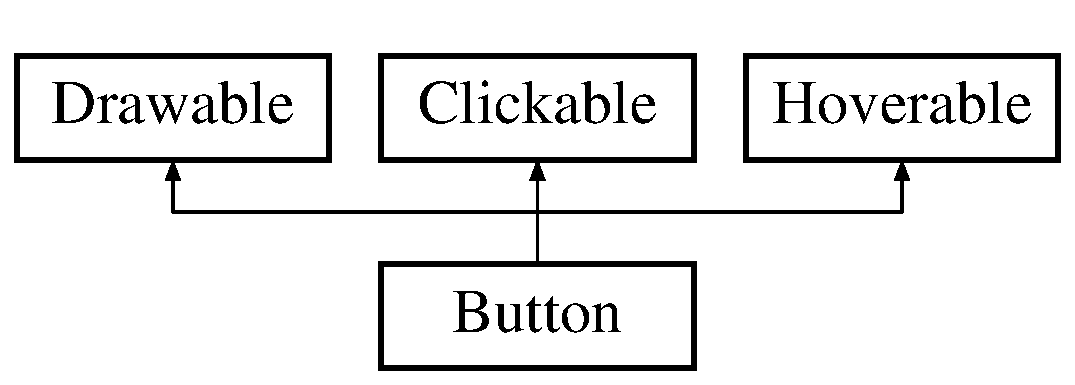
\includegraphics[height=2.000000cm]{class_button}
\end{center}
\end{figure}
\subsection*{Public Member Functions}
\begin{DoxyCompactItemize}
\item 
\hyperlink{class_button_a3b36df1ae23c58aedb9e15a713159459}{Button} ()
\begin{DoxyCompactList}\small\item\em Default Constructor. \end{DoxyCompactList}\item 
\hyperlink{class_button_ad33024be2e6d0cc53e4f11d70ed01c52}{Button} (string text, Vector2f pos, Vector2f size, string texture\+Name)
\begin{DoxyCompactList}\small\item\em Overloaded Constructor. \end{DoxyCompactList}\item 
void \hyperlink{class_button_ada7ed6bfd73ec8704a5d2247c28f6513}{draw} (Render\+Target \&target, Render\+States states) const
\begin{DoxyCompactList}\small\item\em draw function \end{DoxyCompactList}\end{DoxyCompactItemize}
\subsection*{Protected Attributes}
\begin{DoxyCompactItemize}
\item 
\hypertarget{class_button_a353afe3c7c8186bcb6a322d2aa4ab9bc}{}\label{class_button_a353afe3c7c8186bcb6a322d2aa4ab9bc} 
Text \hyperlink{class_button_a353afe3c7c8186bcb6a322d2aa4ab9bc}{m\+\_\+sf\+Button\+Text}
\begin{DoxyCompactList}\small\item\em Text for the button. \end{DoxyCompactList}\item 
\hypertarget{class_button_ab666db59cd6c0d4f281e07d79562ba99}{}\label{class_button_ab666db59cd6c0d4f281e07d79562ba99} 
string \hyperlink{class_button_ab666db59cd6c0d4f281e07d79562ba99}{m\+\_\+s\+Text}
\begin{DoxyCompactList}\small\item\em string contained in the button \end{DoxyCompactList}\item 
\hypertarget{class_button_ac53295dae71348a617af3661b72d39b4}{}\label{class_button_ac53295dae71348a617af3661b72d39b4} 
Texture \hyperlink{class_button_ac53295dae71348a617af3661b72d39b4}{m\+\_\+sf\+Texture}
\begin{DoxyCompactList}\small\item\em Texture for the button. \end{DoxyCompactList}\item 
\hypertarget{class_button_ac8a8b7fa5c8d060205c496ca4610ae25}{}\label{class_button_ac8a8b7fa5c8d060205c496ca4610ae25} 
Sprite \hyperlink{class_button_ac8a8b7fa5c8d060205c496ca4610ae25}{m\+\_\+sf\+Sprite}
\begin{DoxyCompactList}\small\item\em Sprite for the button. \end{DoxyCompactList}\item 
\hypertarget{class_button_a823024f8726bba17b9b092084181d9b7}{}\label{class_button_a823024f8726bba17b9b092084181d9b7} 
Rectangle\+Shape \hyperlink{class_button_a823024f8726bba17b9b092084181d9b7}{m\+\_\+sf\+Rect}
\begin{DoxyCompactList}\small\item\em Rect for the button. \end{DoxyCompactList}\item 
\hypertarget{class_button_a2c351b83dc0d860afc63c015ba598790}{}\label{class_button_a2c351b83dc0d860afc63c015ba598790} 
Font \hyperlink{class_button_a2c351b83dc0d860afc63c015ba598790}{m\+\_\+sf\+Font}
\begin{DoxyCompactList}\small\item\em font for the button \end{DoxyCompactList}\end{DoxyCompactItemize}


\subsection{Detailed Description}
A \hyperlink{class_button}{Button} class.

\hyperlink{class_button}{Button} is an object class that inherests from clicable and drawbale. objects that the user click on should be a \hyperlink{class_button}{Button}. it contains what the text on the button should say and the sprite that will be drawn 
\begin{DoxyCode}
\hyperlink{class_button}{Button} StartGame;
\textcolor{keywordflow}{if}(StartGame.bIsclicked)
\{
Startgame();

\}
\end{DoxyCode}
 

\subsection{Constructor \& Destructor Documentation}
\hypertarget{class_button_a3b36df1ae23c58aedb9e15a713159459}{}\label{class_button_a3b36df1ae23c58aedb9e15a713159459} 
\index{Button@{Button}!Button@{Button}}
\index{Button@{Button}!Button@{Button}}
\subsubsection{\texorpdfstring{Button()}{Button()}\hspace{0.1cm}{\footnotesize\ttfamily [1/2]}}
{\footnotesize\ttfamily Button\+::\+Button (\begin{DoxyParamCaption}{ }\end{DoxyParamCaption})}



Default Constructor. 

Creates an empty button \hypertarget{class_button_ad33024be2e6d0cc53e4f11d70ed01c52}{}\label{class_button_ad33024be2e6d0cc53e4f11d70ed01c52} 
\index{Button@{Button}!Button@{Button}}
\index{Button@{Button}!Button@{Button}}
\subsubsection{\texorpdfstring{Button()}{Button()}\hspace{0.1cm}{\footnotesize\ttfamily [2/2]}}
{\footnotesize\ttfamily Button\+::\+Button (\begin{DoxyParamCaption}\item[{string}]{text,  }\item[{Vector2f}]{pos,  }\item[{Vector2f}]{size,  }\item[{string}]{texture\+Name }\end{DoxyParamCaption})}



Overloaded Constructor. 

Creates the button with its parameteres


\begin{DoxyParams}{Parameters}
{\em text} & string Text that is displayed on the button \\
\hline
{\em pos} & s\+Vector2f position of the button \\
\hline
{\em size} & s\+Vector2f size of the button \\
\hline
\end{DoxyParams}


\subsection{Member Function Documentation}
\hypertarget{class_button_ada7ed6bfd73ec8704a5d2247c28f6513}{}\label{class_button_ada7ed6bfd73ec8704a5d2247c28f6513} 
\index{Button@{Button}!draw@{draw}}
\index{draw@{draw}!Button@{Button}}
\subsubsection{\texorpdfstring{draw()}{draw()}}
{\footnotesize\ttfamily void Button\+::draw (\begin{DoxyParamCaption}\item[{Render\+Target \&}]{target,  }\item[{Render\+States}]{states }\end{DoxyParamCaption}) const}



draw function 

draws the Buttons sprite and text 

The documentation for this class was generated from the following file\+:\begin{DoxyCompactItemize}
\item 
D\+:/\+Uni/\+Year Three/\+Project/\+Product Creation/\+Code/\+Traffic\+Management/\+Default\+S\+F\+M\+L/include/Button.\+h\end{DoxyCompactItemize}

\hypertarget{class_clickable}{}\section{Clickable Class Reference}
\label{class_clickable}\index{Clickable@{Clickable}}
Inheritance diagram for Clickable\+:\begin{figure}[H]
\begin{center}
\leavevmode
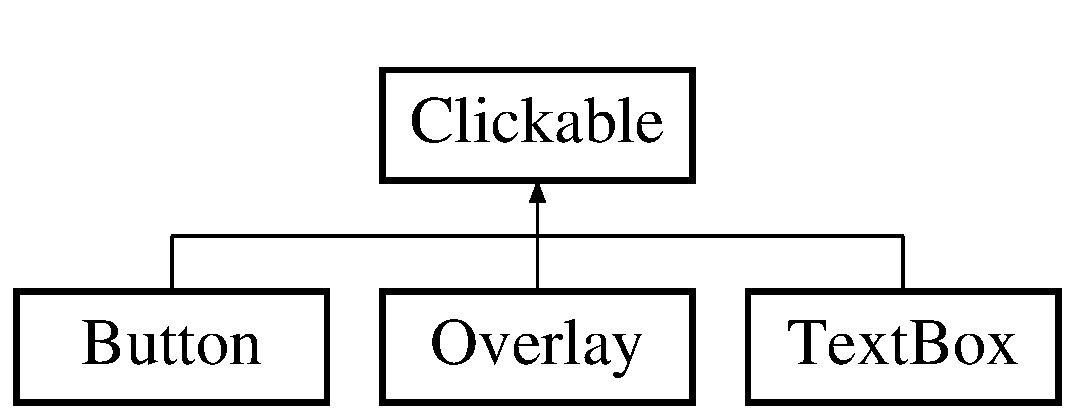
\includegraphics[height=2.000000cm]{class_clickable}
\end{center}
\end{figure}
\subsection*{Public Member Functions}
\begin{DoxyCompactItemize}
\item 
bool \hyperlink{class_clickable_a18e5ca51c572c9cb8a64dced28ccec09}{m\+\_\+b\+Clicked} (Vector2f sf\+Vmouse\+Click)
\begin{DoxyCompactList}\small\item\em Overloaded Bool Function. \end{DoxyCompactList}\end{DoxyCompactItemize}
\subsection*{Protected Attributes}
\begin{DoxyCompactItemize}
\item 
\hypertarget{class_clickable_a220f75f818fc4f3b973c1531044816be}{}\label{class_clickable_a220f75f818fc4f3b973c1531044816be} 
Vector2f \hyperlink{class_clickable_a220f75f818fc4f3b973c1531044816be}{m\+\_\+sf\+V\+Top\+Left\+Pos}
\begin{DoxyCompactList}\small\item\em m\+\_\+sf\+V\+Top\+Left\+Pos sf\+::\+Vector2f where the top left of the button is \end{DoxyCompactList}\item 
\hypertarget{class_clickable_a49ad5930a2e78bd3adfb414115005351}{}\label{class_clickable_a49ad5930a2e78bd3adfb414115005351} 
Vector2f \hyperlink{class_clickable_a49ad5930a2e78bd3adfb414115005351}{m\+\_\+sf\+V\+Size}
\begin{DoxyCompactList}\small\item\em m\+\_\+sf\+V\+Size sf\+::\+Vector2f the size of the button \end{DoxyCompactList}\end{DoxyCompactItemize}


\subsection{Member Function Documentation}
\hypertarget{class_clickable_a18e5ca51c572c9cb8a64dced28ccec09}{}\label{class_clickable_a18e5ca51c572c9cb8a64dced28ccec09} 
\index{Clickable@{Clickable}!m\+\_\+b\+Clicked@{m\+\_\+b\+Clicked}}
\index{m\+\_\+b\+Clicked@{m\+\_\+b\+Clicked}!Clickable@{Clickable}}
\subsubsection{\texorpdfstring{m\+\_\+b\+Clicked()}{m\_bClicked()}}
{\footnotesize\ttfamily bool Clickable\+::m\+\_\+b\+Clicked (\begin{DoxyParamCaption}\item[{Vector2f}]{sf\+Vmouse\+Click }\end{DoxyParamCaption})}



Overloaded Bool Function. 

Testes if the object has been clicked on


\begin{DoxyParams}{Parameters}
{\em sf\+Vmouse\+Click} & sf\+::\+Vector2f of where the mouse was clicked \\
\hline
\end{DoxyParams}


The documentation for this class was generated from the following file\+:\begin{DoxyCompactItemize}
\item 
D\+:/\+Uni/\+Year Three/\+Project/\+Product Creation/\+Code/\+Traffic\+Management/\+Default\+S\+F\+M\+L/include/Clickable.\+h\end{DoxyCompactItemize}

\hypertarget{class_hoverable}{}\section{Hoverable Class Reference}
\label{class_hoverable}\index{Hoverable@{Hoverable}}
Inheritance diagram for Hoverable\+:\begin{figure}[H]
\begin{center}
\leavevmode
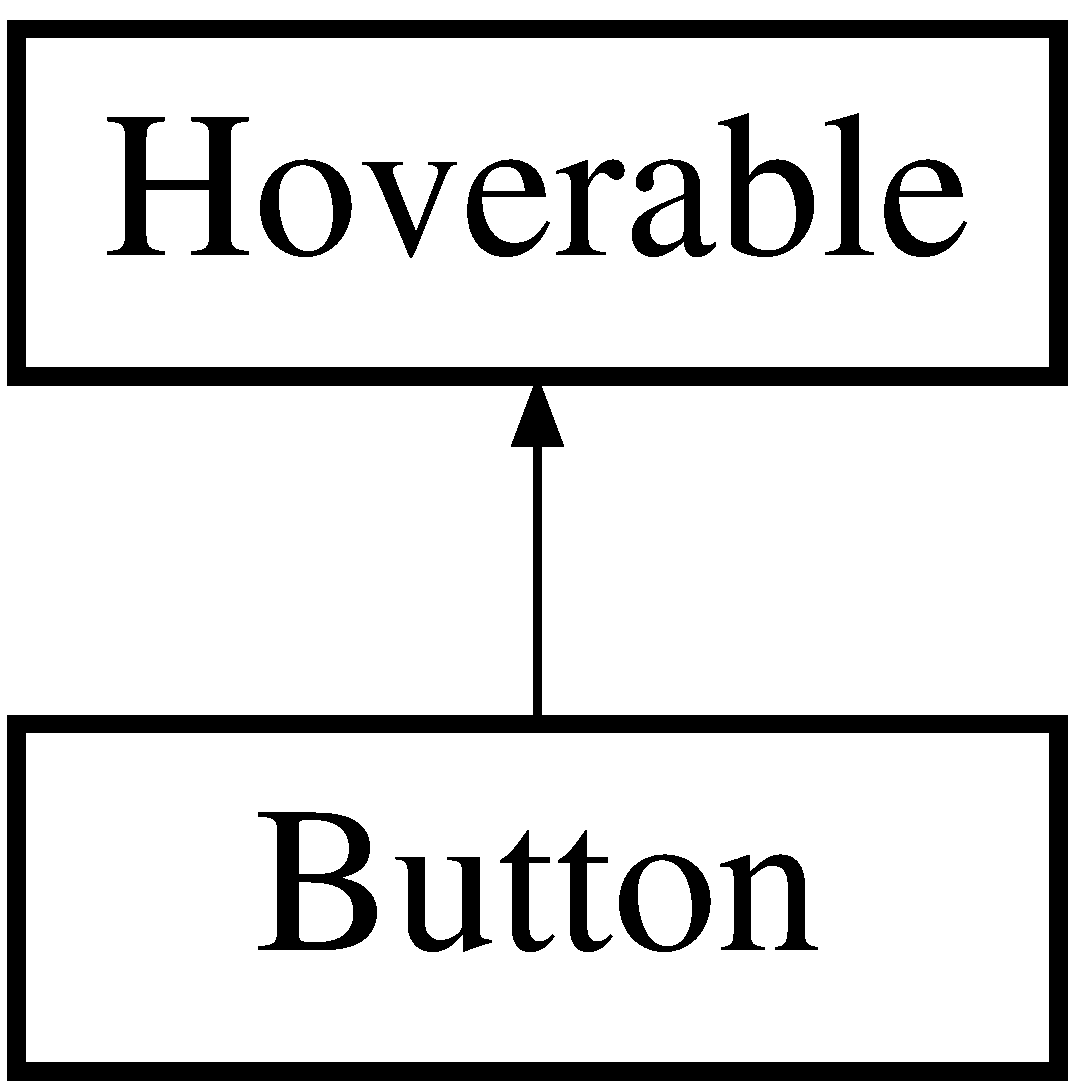
\includegraphics[height=2.000000cm]{class_hoverable}
\end{center}
\end{figure}
\subsection*{Public Member Functions}
\begin{DoxyCompactItemize}
\item 
bool \hyperlink{class_hoverable_a5b2698e36a45fc22a0a45c74608213c5}{m\+\_\+b\+Hovering} (Vector2f sf\+Vmouse\+Click)
\begin{DoxyCompactList}\small\item\em Overloaded Bool Function. \end{DoxyCompactList}\end{DoxyCompactItemize}
\subsection*{Protected Attributes}
\begin{DoxyCompactItemize}
\item 
\hypertarget{class_hoverable_a890c220cc9b6929f72853454aa96cc73}{}\label{class_hoverable_a890c220cc9b6929f72853454aa96cc73} 
Vector2f \hyperlink{class_hoverable_a890c220cc9b6929f72853454aa96cc73}{m\+\_\+sf\+V\+Top\+Left\+Pos\+Hoverable}
\begin{DoxyCompactList}\small\item\em m\+\_\+sf\+V\+Top\+Left\+Pos sf\+::\+Vector2f where the top left of the button is \end{DoxyCompactList}\item 
\hypertarget{class_hoverable_a5134e5e8ed1b8d0d3ba7a0a05fb1f955}{}\label{class_hoverable_a5134e5e8ed1b8d0d3ba7a0a05fb1f955} 
Vector2f \hyperlink{class_hoverable_a5134e5e8ed1b8d0d3ba7a0a05fb1f955}{m\+\_\+sf\+V\+Size\+Hoverable}
\begin{DoxyCompactList}\small\item\em m\+\_\+sf\+V\+Size sf\+::\+Vector2f the size of the button \end{DoxyCompactList}\end{DoxyCompactItemize}


\subsection{Detailed Description}
A \hyperlink{class_hoverable}{Hoverable} class.

\hyperlink{_hoverable_8h_source}{Hoverable.\+h} is a blass class that will be used to test if an element is been hovered on by the mouse Objects that can be hovered on should inherit from \hyperlink{_hoverable_8h_source}{Hoverable.\+h} It contains public bool fuction that should be used to test is sometimes has been hovered over 
\begin{DoxyCode}
\hyperlink{class_button}{Button} StartGame;
\textcolor{keywordflow}{if}(StartGame.bIsclicked)
\{
    \textcolor{keywordflow}{if}(button01.m\_bHovering(mousePosition)) hint.open();

\}
\end{DoxyCode}
 

\subsection{Member Function Documentation}
\hypertarget{class_hoverable_a5b2698e36a45fc22a0a45c74608213c5}{}\label{class_hoverable_a5b2698e36a45fc22a0a45c74608213c5} 
\index{Hoverable@{Hoverable}!m\+\_\+b\+Hovering@{m\+\_\+b\+Hovering}}
\index{m\+\_\+b\+Hovering@{m\+\_\+b\+Hovering}!Hoverable@{Hoverable}}
\subsubsection{\texorpdfstring{m\+\_\+b\+Hovering()}{m\_bHovering()}}
{\footnotesize\ttfamily bool Hoverable\+::m\+\_\+b\+Hovering (\begin{DoxyParamCaption}\item[{Vector2f}]{sf\+Vmouse\+Click }\end{DoxyParamCaption})}



Overloaded Bool Function. 

Testes if the object has been clicked on


\begin{DoxyParams}{Parameters}
{\em sf\+Vmouse\+Click} & sf\+::\+Vector2f of where the mouse is hovering \\
\hline
\end{DoxyParams}


The documentation for this class was generated from the following file\+:\begin{DoxyCompactItemize}
\item 
D\+:/\+Uni/\+Year Three/\+Project/\+Product Creation/\+Code/\+Traffic\+Management/\+Default\+S\+F\+M\+L/include/Hoverable.\+h\end{DoxyCompactItemize}

\hypertarget{class_overlay}{}\section{Overlay Class Reference}
\label{class_overlay}\index{Overlay@{Overlay}}
Inheritance diagram for Overlay\+:\begin{figure}[H]
\begin{center}
\leavevmode
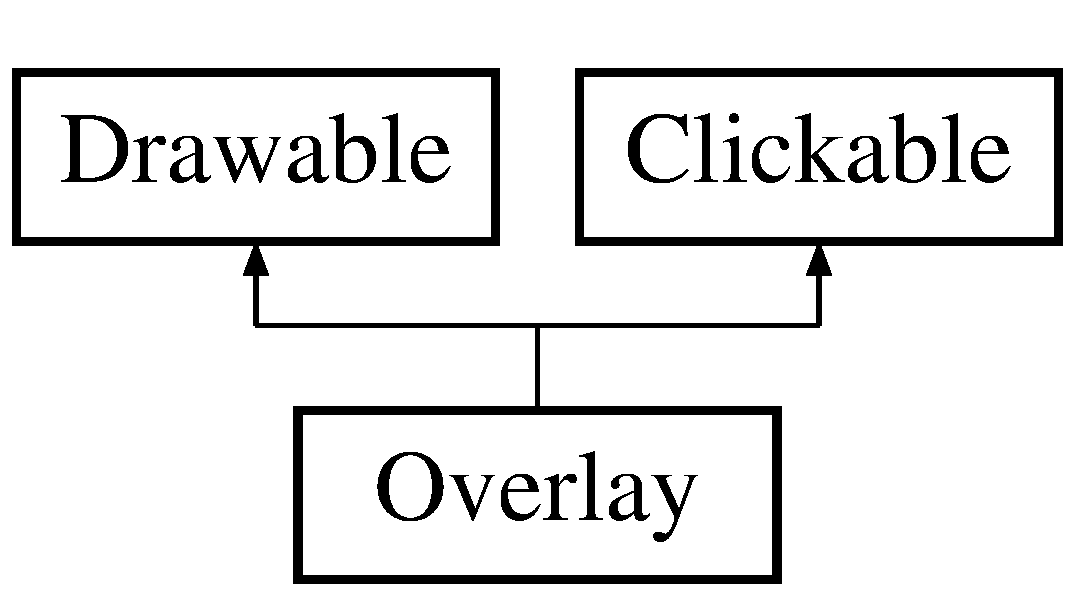
\includegraphics[height=2.000000cm]{class_overlay}
\end{center}
\end{figure}
\subsection*{Classes}
\begin{DoxyCompactItemize}
\item 
class \hyperlink{class_overlay_1_1h}{h}
\end{DoxyCompactItemize}
\subsection*{Public Member Functions}
\begin{DoxyCompactItemize}
\item 
\hyperlink{class_overlay_ab4f509d502931bcaad03418470993d70}{Overlay} ()
\begin{DoxyCompactList}\small\item\em Default Constructor. \end{DoxyCompactList}\item 
\hyperlink{class_overlay_a6cd84b6dc4fdcb2a6fbfafaf5e63e170}{Overlay} (Vector2f position, Vector2f size, string text)
\begin{DoxyCompactList}\small\item\em Overloaded Constructor. \end{DoxyCompactList}\item 
void \hyperlink{class_overlay_abe32d7e0e71733150f7a28cf3e851aa1}{draw} (Render\+Target \&target, Render\+States states) const
\begin{DoxyCompactList}\small\item\em draw function \end{DoxyCompactList}\end{DoxyCompactItemize}
\subsection*{Public Attributes}
\begin{DoxyCompactItemize}
\item 
\hypertarget{class_overlay_a9a70a96aa1bc41ee3e0c34dfb705f7b9}{}\label{class_overlay_a9a70a96aa1bc41ee3e0c34dfb705f7b9} 
bool \hyperlink{class_overlay_a9a70a96aa1bc41ee3e0c34dfb705f7b9}{m\+\_\+b\+Draw} = true
\begin{DoxyCompactList}\small\item\em Bool to control drawing of overlay. \end{DoxyCompactList}\end{DoxyCompactItemize}
\subsection*{Additional Inherited Members}


\subsection{Constructor \& Destructor Documentation}
\hypertarget{class_overlay_ab4f509d502931bcaad03418470993d70}{}\label{class_overlay_ab4f509d502931bcaad03418470993d70} 
\index{Overlay@{Overlay}!Overlay@{Overlay}}
\index{Overlay@{Overlay}!Overlay@{Overlay}}
\subsubsection{\texorpdfstring{Overlay()}{Overlay()}\hspace{0.1cm}{\footnotesize\ttfamily [1/2]}}
{\footnotesize\ttfamily Overlay\+::\+Overlay (\begin{DoxyParamCaption}{ }\end{DoxyParamCaption})}



Default Constructor. 

Creates an empty overlay \hypertarget{class_overlay_a6cd84b6dc4fdcb2a6fbfafaf5e63e170}{}\label{class_overlay_a6cd84b6dc4fdcb2a6fbfafaf5e63e170} 
\index{Overlay@{Overlay}!Overlay@{Overlay}}
\index{Overlay@{Overlay}!Overlay@{Overlay}}
\subsubsection{\texorpdfstring{Overlay()}{Overlay()}\hspace{0.1cm}{\footnotesize\ttfamily [2/2]}}
{\footnotesize\ttfamily Overlay\+::\+Overlay (\begin{DoxyParamCaption}\item[{Vector2f}]{position,  }\item[{Vector2f}]{size,  }\item[{string}]{text }\end{DoxyParamCaption})}



Overloaded Constructor. 

Creates an overlay with the following parameters


\begin{DoxyParams}{Parameters}
{\em vector2f} & postition position of overlay \\
\hline
{\em vector2f} & size size of the overlay \\
\hline
{\em string} & text for the overlay \\
\hline
\end{DoxyParams}


\subsection{Member Function Documentation}
\hypertarget{class_overlay_abe32d7e0e71733150f7a28cf3e851aa1}{}\label{class_overlay_abe32d7e0e71733150f7a28cf3e851aa1} 
\index{Overlay@{Overlay}!draw@{draw}}
\index{draw@{draw}!Overlay@{Overlay}}
\subsubsection{\texorpdfstring{draw()}{draw()}}
{\footnotesize\ttfamily void Overlay\+::draw (\begin{DoxyParamCaption}\item[{Render\+Target \&}]{target,  }\item[{Render\+States}]{states }\end{DoxyParamCaption}) const}



draw function 

draws the overlay and button 

The documentation for this class was generated from the following file\+:\begin{DoxyCompactItemize}
\item 
D\+:/\+Uni/\+Year Three/\+Project/\+Product Creation/\+Code/\+Traffic\+Management/\+Default\+S\+F\+M\+L/include/Overlay.\+h\end{DoxyCompactItemize}

\hypertarget{class_profile}{}\section{Profile Class Reference}
\label{class_profile}\index{Profile@{Profile}}
\subsection*{Classes}
\begin{DoxyCompactItemize}
\item 
class \hyperlink{class_profile_1_1h}{h}
\end{DoxyCompactItemize}
\subsection*{Public Member Functions}
\begin{DoxyCompactItemize}
\item 
\hyperlink{class_profile_a4eea708cdbed0262d9e7ddbe3f1e3f89}{Profile} ()
\begin{DoxyCompactList}\small\item\em Default Constructor. \end{DoxyCompactList}\item 
\hyperlink{class_profile_a2f1ced1b7bf7fc6d54468f645ba9899c}{Profile} (string location)
\begin{DoxyCompactList}\small\item\em Overloaded Constructor. \end{DoxyCompactList}\item 
\hyperlink{class_profile_a69b3d3c58a1db8e6edeea0c48f40ab4b}{Profile} (string name\+Of\+Player, bool create)
\begin{DoxyCompactList}\small\item\em Overloaded Constructor. \end{DoxyCompactList}\item 
\hyperlink{class_profile_a58fa758a59bc4ee3c1a9980e360e4e98}{$\sim$\+Profile} ()
\begin{DoxyCompactList}\small\item\em Default de\+Constructor. \end{DoxyCompactList}\item 
\hypertarget{class_profile_a21c59434bd6dec62c974b208caf2ff58}{}\label{class_profile_a21c59434bd6dec62c974b208caf2ff58} 
void \hyperlink{class_profile_a21c59434bd6dec62c974b208caf2ff58}{save\+Profile} ()
\begin{DoxyCompactList}\small\item\em fuction to save the content of the profile to a text file \end{DoxyCompactList}\item 
\hypertarget{class_profile_afe06c4b329f11dce5478f17c201a0dff}{}\label{class_profile_afe06c4b329f11dce5478f17c201a0dff} 
void \hyperlink{class_profile_afe06c4b329f11dce5478f17c201a0dff}{load\+Profile} (string name)
\begin{DoxyCompactList}\small\item\em fuction to load the content of a text file to the profile \end{DoxyCompactList}\item 
\hypertarget{class_profile_ac1e3c9978e12cb532f5a9582a735d990}{}\label{class_profile_ac1e3c9978e12cb532f5a9582a735d990} 
void \hyperlink{class_profile_ac1e3c9978e12cb532f5a9582a735d990}{delete\+Profile} (string name)
\begin{DoxyCompactList}\small\item\em fuction to delete a profile \end{DoxyCompactList}\end{DoxyCompactItemize}
\subsection*{Public Attributes}
\begin{DoxyCompactItemize}
\item 
\hypertarget{class_profile_a5f0bae7cea5466440b5175a418909db7}{}\label{class_profile_a5f0bae7cea5466440b5175a418909db7} 
string \hyperlink{class_profile_a5f0bae7cea5466440b5175a418909db7}{m\+\_\+s\+Profile\+Name}
\begin{DoxyCompactList}\small\item\em Name of the player using profile. \end{DoxyCompactList}\item 
\hypertarget{class_profile_af0e3b9cdcf409029d4dbedeb08c556d6}{}\label{class_profile_af0e3b9cdcf409029d4dbedeb08c556d6} 
unsigned int \hyperlink{class_profile_af0e3b9cdcf409029d4dbedeb08c556d6}{m\+\_\+uilevel}
\begin{DoxyCompactList}\small\item\em Level of the player. \end{DoxyCompactList}\item 
\hypertarget{class_profile_a80b39b98107c13ddb7b0cc22f62f9a9d}{}\label{class_profile_a80b39b98107c13ddb7b0cc22f62f9a9d} 
float \hyperlink{class_profile_a80b39b98107c13ddb7b0cc22f62f9a9d}{m\+\_\+f\+XP}
\begin{DoxyCompactList}\small\item\em how much experience the player has earned \end{DoxyCompactList}\item 
\hypertarget{class_profile_abe8f54c015b06ad58f59d59fcca02bad}{}\label{class_profile_abe8f54c015b06ad58f59d59fcca02bad} 
unsigned int \hyperlink{class_profile_abe8f54c015b06ad58f59d59fcca02bad}{m\+\_\+ui\+Pedestrians\+Total}
\begin{DoxyCompactList}\small\item\em total of how many pedestrians player has passed through a level \end{DoxyCompactList}\item 
\hypertarget{class_profile_a735b68ae846ce7fe33adc71ddf7ae301}{}\label{class_profile_a735b68ae846ce7fe33adc71ddf7ae301} 
unsigned int \hyperlink{class_profile_a735b68ae846ce7fe33adc71ddf7ae301}{m\+\_\+ui\+Cars\+Total}
\begin{DoxyCompactList}\small\item\em total of how many cars player has passed through a level \end{DoxyCompactList}\item 
\hypertarget{class_profile_aca84c340c094843682075f6d8798b1a7}{}\label{class_profile_aca84c340c094843682075f6d8798b1a7} 
unsigned int \hyperlink{class_profile_aca84c340c094843682075f6d8798b1a7}{m\+\_\+ui\+Crashes\+Total}
\begin{DoxyCompactList}\small\item\em total of how many crashes the the player has experienced \end{DoxyCompactList}\item 
\hypertarget{class_profile_af340a69fb34e4bc00394d4d644d286f5}{}\label{class_profile_af340a69fb34e4bc00394d4d644d286f5} 
unsigned int \hyperlink{class_profile_af340a69fb34e4bc00394d4d644d286f5}{m\+\_\+ui\+Fatalities\+Total}
\begin{DoxyCompactList}\small\item\em total of how many pedestrains are hit by cars \end{DoxyCompactList}\item 
\hypertarget{class_profile_aa542d28bec2f4eed0e79f01428e7b88c}{}\label{class_profile_aa542d28bec2f4eed0e79f01428e7b88c} 
float \hyperlink{class_profile_aa542d28bec2f4eed0e79f01428e7b88c}{m\+\_\+f\+Flow\+Rate}
\begin{DoxyCompactList}\small\item\em average of how many cars make it through a level in a minute \end{DoxyCompactList}\item 
\hypertarget{class_profile_ad6d078cfa75a1e6ac7351f724a48116b}{}\label{class_profile_ad6d078cfa75a1e6ac7351f724a48116b} 
float \hyperlink{class_profile_ad6d078cfa75a1e6ac7351f724a48116b}{m\+\_\+f\+Pass\+Rate} = (\hyperlink{class_profile_a735b68ae846ce7fe33adc71ddf7ae301}{m\+\_\+ui\+Cars\+Total} + \hyperlink{class_profile_abe8f54c015b06ad58f59d59fcca02bad}{m\+\_\+ui\+Pedestrians\+Total}) / ((\hyperlink{class_profile_aca84c340c094843682075f6d8798b1a7}{m\+\_\+ui\+Crashes\+Total} + \hyperlink{class_profile_af340a69fb34e4bc00394d4d644d286f5}{m\+\_\+ui\+Fatalities\+Total})+1)
\begin{DoxyCompactList}\small\item\em ratio of passed cars/pedestrians against crashes and fatalities \end{DoxyCompactList}\item 
\hypertarget{class_profile_abe25a6803a857da40de321b06be657d5}{}\label{class_profile_abe25a6803a857da40de321b06be657d5} 
int \hyperlink{class_profile_abe25a6803a857da40de321b06be657d5}{m\+\_\+i\+Game\+Audio\+Volume}
\begin{DoxyCompactList}\small\item\em game audio level \end{DoxyCompactList}\item 
\hypertarget{class_profile_a4d785b3d9bd75173abfa6f8b98d72f70}{}\label{class_profile_a4d785b3d9bd75173abfa6f8b98d72f70} 
int \hyperlink{class_profile_a4d785b3d9bd75173abfa6f8b98d72f70}{m\+\_\+i\+Interface\+Audio\+Volume}
\begin{DoxyCompactList}\small\item\em interface audio level \end{DoxyCompactList}\item 
\hypertarget{class_profile_ad539b144e98e879f6759a9082ad8f17c}{}\label{class_profile_ad539b144e98e879f6759a9082ad8f17c} 
int \hyperlink{class_profile_ad539b144e98e879f6759a9082ad8f17c}{m\+\_\+i\+Music\+Audio\+Volume}
\begin{DoxyCompactList}\small\item\em music audio level \end{DoxyCompactList}\item 
\hypertarget{class_profile_a32263f8c1a2c9d2158450774601f77b8}{}\label{class_profile_a32263f8c1a2c9d2158450774601f77b8} 
Vector2f \hyperlink{class_profile_a32263f8c1a2c9d2158450774601f77b8}{m\+\_\+sf\+Resolution}
\begin{DoxyCompactList}\small\item\em Graphics Resolution ( x , y) \end{DoxyCompactList}\item 
\hypertarget{class_profile_a46c194b7ca443a11e74c413b7f4795bd}{}\label{class_profile_a46c194b7ca443a11e74c413b7f4795bd} 
bool \hyperlink{class_profile_a46c194b7ca443a11e74c413b7f4795bd}{m\+\_\+b\+Fullscreen}
\begin{DoxyCompactList}\small\item\em Fullscreen boolean. \end{DoxyCompactList}\item 
\hypertarget{class_profile_abe8d5282ca1966bf2985bf4d79bef78f}{}\label{class_profile_abe8d5282ca1966bf2985bf4d79bef78f} 
bool \hyperlink{class_profile_abe8d5282ca1966bf2985bf4d79bef78f}{m\+\_\+b\+Textures}
\begin{DoxyCompactList}\small\item\em high quality texures boolean \end{DoxyCompactList}\end{DoxyCompactItemize}


\subsection{Constructor \& Destructor Documentation}
\hypertarget{class_profile_a4eea708cdbed0262d9e7ddbe3f1e3f89}{}\label{class_profile_a4eea708cdbed0262d9e7ddbe3f1e3f89} 
\index{Profile@{Profile}!Profile@{Profile}}
\index{Profile@{Profile}!Profile@{Profile}}
\subsubsection{\texorpdfstring{Profile()}{Profile()}\hspace{0.1cm}{\footnotesize\ttfamily [1/3]}}
{\footnotesize\ttfamily Profile\+::\+Profile (\begin{DoxyParamCaption}{ }\end{DoxyParamCaption})}



Default Constructor. 

Creates an empty \hyperlink{class_profile}{Profile} \hypertarget{class_profile_a2f1ced1b7bf7fc6d54468f645ba9899c}{}\label{class_profile_a2f1ced1b7bf7fc6d54468f645ba9899c} 
\index{Profile@{Profile}!Profile@{Profile}}
\index{Profile@{Profile}!Profile@{Profile}}
\subsubsection{\texorpdfstring{Profile()}{Profile()}\hspace{0.1cm}{\footnotesize\ttfamily [2/3]}}
{\footnotesize\ttfamily Profile\+::\+Profile (\begin{DoxyParamCaption}\item[{string}]{location }\end{DoxyParamCaption})}



Overloaded Constructor. 

\hyperlink{class_profile}{Profile}


\begin{DoxyParams}{Parameters}
{\em location} & string path to the profile \\
\hline
\end{DoxyParams}
\hypertarget{class_profile_a69b3d3c58a1db8e6edeea0c48f40ab4b}{}\label{class_profile_a69b3d3c58a1db8e6edeea0c48f40ab4b} 
\index{Profile@{Profile}!Profile@{Profile}}
\index{Profile@{Profile}!Profile@{Profile}}
\subsubsection{\texorpdfstring{Profile()}{Profile()}\hspace{0.1cm}{\footnotesize\ttfamily [3/3]}}
{\footnotesize\ttfamily Profile\+::\+Profile (\begin{DoxyParamCaption}\item[{string}]{name\+Of\+Player,  }\item[{bool}]{create }\end{DoxyParamCaption})}



Overloaded Constructor. 

\hyperlink{class_profile}{Profile}


\begin{DoxyParams}{Parameters}
{\em location} & string path to the profile \\
\hline
{\em create} & bool wheather to create new file or not \\
\hline
\end{DoxyParams}
\hypertarget{class_profile_a58fa758a59bc4ee3c1a9980e360e4e98}{}\label{class_profile_a58fa758a59bc4ee3c1a9980e360e4e98} 
\index{Profile@{Profile}!````~Profile@{$\sim$\+Profile}}
\index{````~Profile@{$\sim$\+Profile}!Profile@{Profile}}
\subsubsection{\texorpdfstring{$\sim$\+Profile()}{~Profile()}}
{\footnotesize\ttfamily Profile\+::$\sim$\+Profile (\begin{DoxyParamCaption}{ }\end{DoxyParamCaption})}



Default de\+Constructor. 

Deletes the profile 

The documentation for this class was generated from the following file\+:\begin{DoxyCompactItemize}
\item 
D\+:/\+Uni/\+Year Three/\+Project/\+Product Creation/\+Code/\+Traffic\+Management/\+Default\+S\+F\+M\+L/include/Profile.\+h\end{DoxyCompactItemize}

\hypertarget{class_text_box}{}\section{Text\+Box Class Reference}
\label{class_text_box}\index{Text\+Box@{Text\+Box}}
Inheritance diagram for Text\+Box\+:\begin{figure}[H]
\begin{center}
\leavevmode
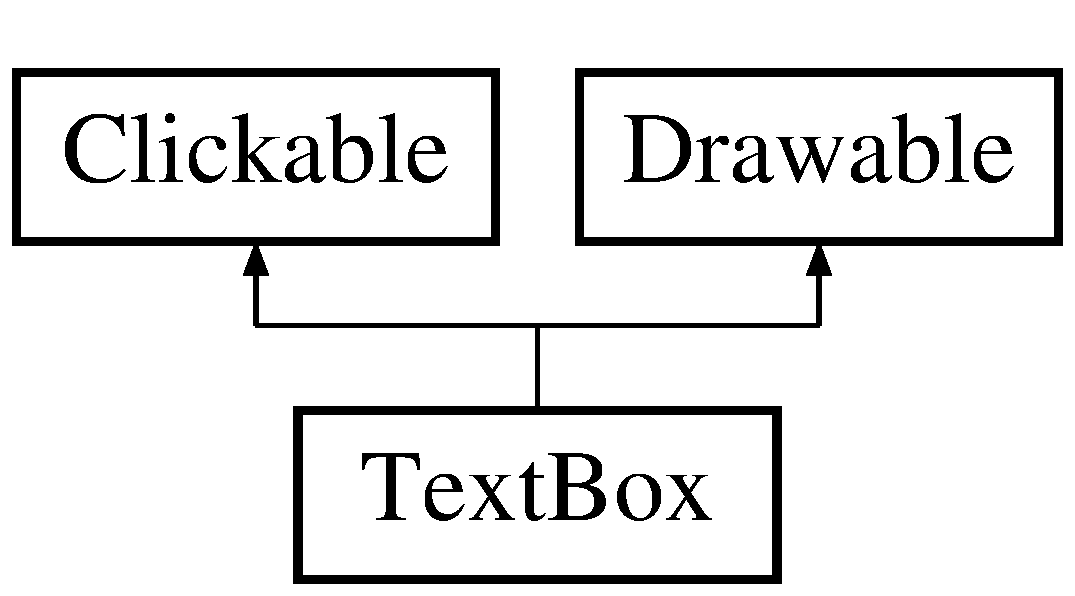
\includegraphics[height=2.000000cm]{class_text_box}
\end{center}
\end{figure}
\subsection*{Public Member Functions}
\begin{DoxyCompactItemize}
\item 
\hyperlink{class_text_box_a25b67e5ff6788c60b8aef3f3540879d0}{Text\+Box} ()
\begin{DoxyCompactList}\small\item\em Default Constructor. \end{DoxyCompactList}\item 
\hyperlink{class_text_box_a9df04c5eb70d4d6b75907c56ecce6d8e}{Text\+Box} (string text, Vector2f pos, Vector2f size, string texture\+Name)
\begin{DoxyCompactList}\small\item\em Overloaded Constructor. \end{DoxyCompactList}\item 
\hyperlink{class_text_box_ac3cc88a3ac171658ebaf44b01f4adf80}{$\sim$\+Text\+Box} ()
\begin{DoxyCompactList}\small\item\em Default de\+Constructor. \end{DoxyCompactList}\item 
void \hyperlink{class_text_box_a9139c31dc807fa0c478215086f3fc7f1}{take\+Input} (Keyboard\+::\+Key pressed\+Key)
\begin{DoxyCompactList}\small\item\em Processes key presses while button is selected. \end{DoxyCompactList}\item 
void \hyperlink{class_text_box_a94f8b1fa218dabaaf892388cbf8df1fa}{draw} (Render\+Target \&target, Render\+States states) const
\begin{DoxyCompactList}\small\item\em draw function \end{DoxyCompactList}\end{DoxyCompactItemize}
\subsection*{Public Attributes}
\begin{DoxyCompactItemize}
\item 
\hypertarget{class_text_box_a9bd587d5dda491ff96bb5ef4497eb406}{}\label{class_text_box_a9bd587d5dda491ff96bb5ef4497eb406} 
bool \hyperlink{class_text_box_a9bd587d5dda491ff96bb5ef4497eb406}{m\+\_\+b\+Is\+Entering} = false
\begin{DoxyCompactList}\small\item\em bool for entering text \end{DoxyCompactList}\item 
\hypertarget{class_text_box_a79dde249421f3a5b26f52bbf59f9f2c3}{}\label{class_text_box_a79dde249421f3a5b26f52bbf59f9f2c3} 
String \hyperlink{class_text_box_a79dde249421f3a5b26f52bbf59f9f2c3}{m\+\_\+s\+Text}
\begin{DoxyCompactList}\small\item\em string for the text \end{DoxyCompactList}\end{DoxyCompactItemize}
\subsection*{Additional Inherited Members}


\subsection{Constructor \& Destructor Documentation}
\hypertarget{class_text_box_a25b67e5ff6788c60b8aef3f3540879d0}{}\label{class_text_box_a25b67e5ff6788c60b8aef3f3540879d0} 
\index{Text\+Box@{Text\+Box}!Text\+Box@{Text\+Box}}
\index{Text\+Box@{Text\+Box}!Text\+Box@{Text\+Box}}
\subsubsection{\texorpdfstring{Text\+Box()}{TextBox()}\hspace{0.1cm}{\footnotesize\ttfamily [1/2]}}
{\footnotesize\ttfamily Text\+Box\+::\+Text\+Box (\begin{DoxyParamCaption}{ }\end{DoxyParamCaption})}



Default Constructor. 

Creates an empty \hyperlink{class_text_box}{Text\+Box} \hypertarget{class_text_box_a9df04c5eb70d4d6b75907c56ecce6d8e}{}\label{class_text_box_a9df04c5eb70d4d6b75907c56ecce6d8e} 
\index{Text\+Box@{Text\+Box}!Text\+Box@{Text\+Box}}
\index{Text\+Box@{Text\+Box}!Text\+Box@{Text\+Box}}
\subsubsection{\texorpdfstring{Text\+Box()}{TextBox()}\hspace{0.1cm}{\footnotesize\ttfamily [2/2]}}
{\footnotesize\ttfamily Text\+Box\+::\+Text\+Box (\begin{DoxyParamCaption}\item[{string}]{text,  }\item[{Vector2f}]{pos,  }\item[{Vector2f}]{size,  }\item[{string}]{texture\+Name }\end{DoxyParamCaption})}



Overloaded Constructor. 

Creates the \hyperlink{class_text_box}{Text\+Box} with its parameteres


\begin{DoxyParams}{Parameters}
{\em text} & string Text that is displayed on the \hyperlink{class_text_box}{Text\+Box} \\
\hline
{\em pos} & s\+Vector2f position of the \hyperlink{class_text_box}{Text\+Box} \\
\hline
{\em size} & s\+Vector2f size of the \hyperlink{class_text_box}{Text\+Box} \\
\hline
\end{DoxyParams}
\hypertarget{class_text_box_ac3cc88a3ac171658ebaf44b01f4adf80}{}\label{class_text_box_ac3cc88a3ac171658ebaf44b01f4adf80} 
\index{Text\+Box@{Text\+Box}!````~Text\+Box@{$\sim$\+Text\+Box}}
\index{````~Text\+Box@{$\sim$\+Text\+Box}!Text\+Box@{Text\+Box}}
\subsubsection{\texorpdfstring{$\sim$\+Text\+Box()}{~TextBox()}}
{\footnotesize\ttfamily Text\+Box\+::$\sim$\+Text\+Box (\begin{DoxyParamCaption}{ }\end{DoxyParamCaption})}



Default de\+Constructor. 

Deletes the text\+Box 

\subsection{Member Function Documentation}
\hypertarget{class_text_box_a94f8b1fa218dabaaf892388cbf8df1fa}{}\label{class_text_box_a94f8b1fa218dabaaf892388cbf8df1fa} 
\index{Text\+Box@{Text\+Box}!draw@{draw}}
\index{draw@{draw}!Text\+Box@{Text\+Box}}
\subsubsection{\texorpdfstring{draw()}{draw()}}
{\footnotesize\ttfamily void Text\+Box\+::draw (\begin{DoxyParamCaption}\item[{Render\+Target \&}]{target,  }\item[{Render\+States}]{states }\end{DoxyParamCaption}) const}



draw function 

draws the Buttons sprite and text \hypertarget{class_text_box_a9139c31dc807fa0c478215086f3fc7f1}{}\label{class_text_box_a9139c31dc807fa0c478215086f3fc7f1} 
\index{Text\+Box@{Text\+Box}!take\+Input@{take\+Input}}
\index{take\+Input@{take\+Input}!Text\+Box@{Text\+Box}}
\subsubsection{\texorpdfstring{take\+Input()}{takeInput()}}
{\footnotesize\ttfamily void Text\+Box\+::take\+Input (\begin{DoxyParamCaption}\item[{Keyboard\+::\+Key}]{pressed\+Key }\end{DoxyParamCaption})}



Processes key presses while button is selected. 

If valid charachter add to string if enter complete string if escape clear string


\begin{DoxyParams}{Parameters}
{\em } & \\
\hline
\end{DoxyParams}


The documentation for this class was generated from the following file\+:\begin{DoxyCompactItemize}
\item 
D\+:/\+Uni/\+Year Three/\+Project/\+Product Creation/\+Code/\+Traffic\+Management/\+Default\+S\+F\+M\+L/include/Text\+Box.\+h\end{DoxyCompactItemize}

%--- End generated contents ---

% Index
\backmatter
\newpage
\phantomsection
\clearemptydoublepage
\addcontentsline{toc}{chapter}{Index}
\printindex

\end{document}
